\documentclass[12pt]{article}

\usepackage{graphicx}
\usepackage{listings}
\usepackage{hyperref}
\usepackage{float}
\usepackage{enumitem}

\graphicspath{ {./images/} }

\oddsidemargin 0mm
\evensidemargin 0mm
\textwidth 160mm
\textheight 200mm

\pagestyle {plain}
\pagenumbering{arabic}

\newcounter{stepnum}

\title{CS/SE 2XC3 Lab 7 Report}
\author{
  Glotov, Oleg\\ L03, 400174037\\
  \texttt{glotovo@mcmaster.ca}
  \and
  Willson, Emma\\ L02, 400309856\\
  \texttt{willsone@mcmaster.ca}
  }
\date{\today}

\begin{document}

\maketitle

This report includes the main observations that we found in this week's lab, along with the analysis of our results.

\newpage 
\section{Basic Graph Algorithms}
In this section, we discuss basic graph operations and their implementations. 
\subsection{Generating Random Graphs}
We defined a function \verb+create_random_graph(n,c)+ to randomly construct a graph when given some number of nodes $n$ and number of edges $c$. The argument $c$ is given the upper bound $\frac{n\times(n-1)}{2}$ because there can be at most $\frac{n\times(n-1)}{2}$ unique edges in a graph with $n$ nodes. The algorithm initializes a graph with $n$ nodes and then generates a candidate edge between two randomly selected nodes. The candidate edge is accepted only if it is between two unique nodes (does not accept self-loops) and only if it (or its reverse) does not already exist in the graph. If a candidate edge is invalid, it is discarded and the algorithm randomly generates another one. The algorithm adds $c$ valid edges to the graph and returns the populated graph.
\subsection{Cycles Probability}
Our \verb+has_cycle(G)+ function checks if a given graph $G$ contains one or more cycles using a variation on our DFS3 algorithm. If the input graph is connected, the algorithm starts at node $0$ because all nodes are accessible from any other node. If it is not connected, the algorithm checks for a cycle beginning at each node in the graph. The algorithm traverses the graph depth-first, marking visited nodes. When visiting a node, the current node and its parent are popped from the stack and the algorithm moves on to each node adjacent to the current node. If an adjacent node is unvisited, it is marked and the current and adjacent node are pushed onto the stack. If an adjacent node has been visited but is not the current node's parent, then there is a cycle and the algorithm returns true.
\subsection{Connected Probability}
The complexities of the various implementations can be seen in the graph below.
\begin{figure}[H]
\centering
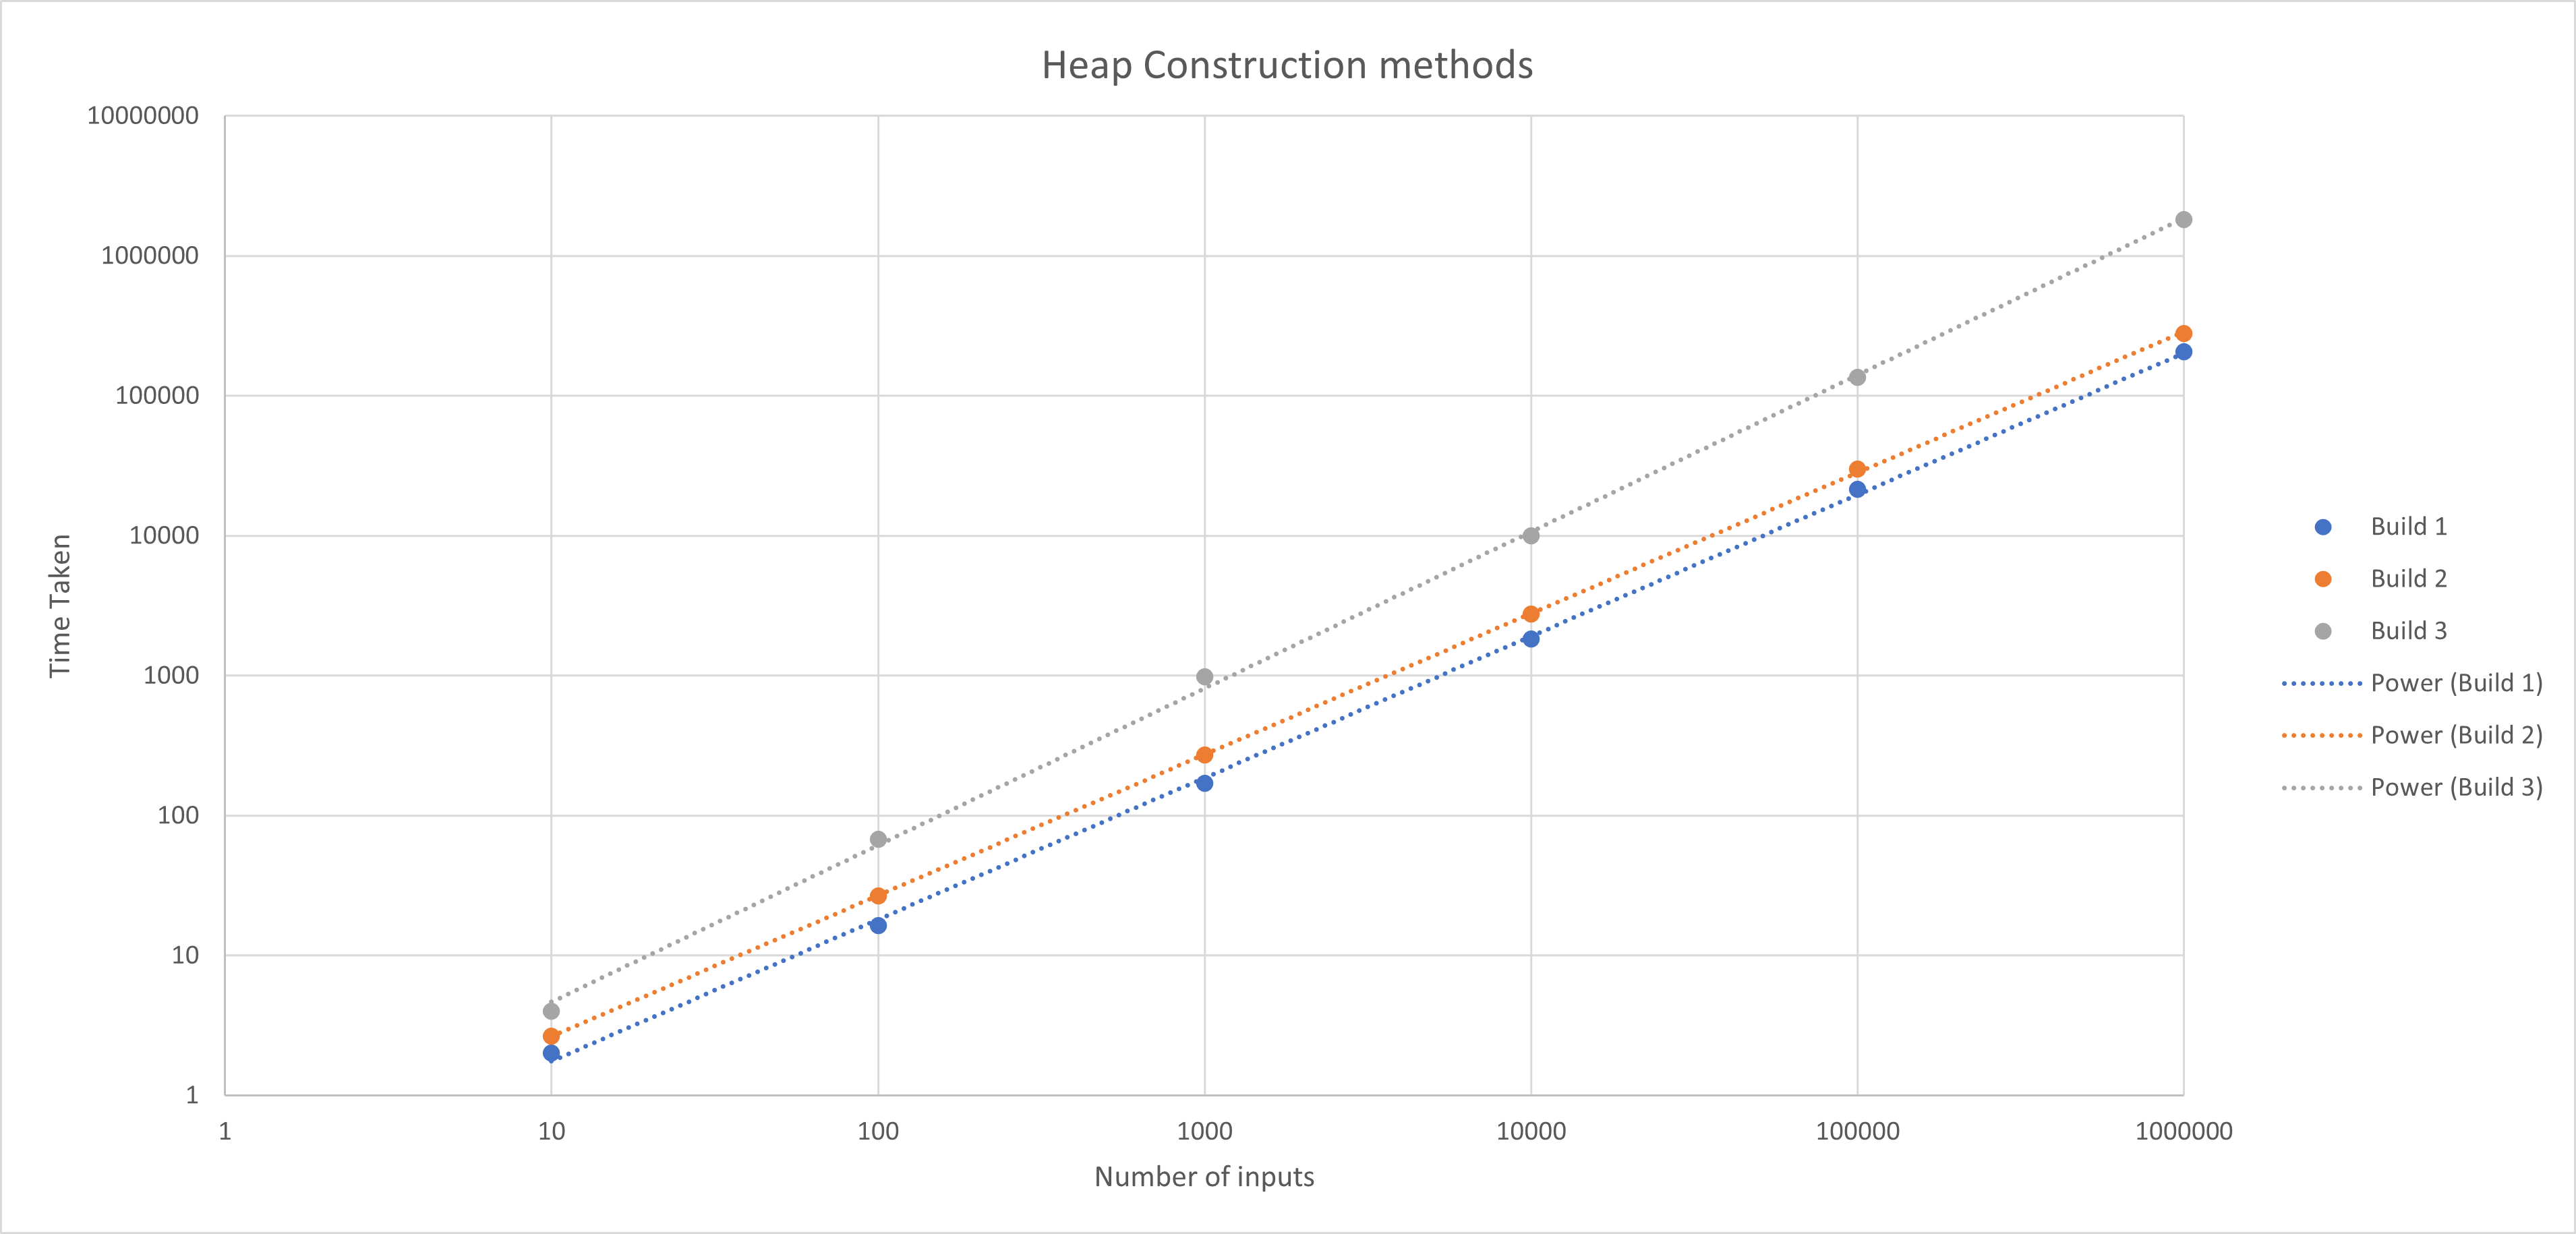
\includegraphics[width=0.9\textwidth,height=\textheight,keepaspectratio]{heap}
\caption{performance of three implementations}
\label{Figure: m1}
\end{figure}

\end{document}

